\section*{FirstClass Functions}

Consider the Lambda Calculus. It has variables, functions and function application. The only values are (closed) functions. Instead of \texttt{(fun x -> e)} we write: $\lambda x. e$

\begin{center}
	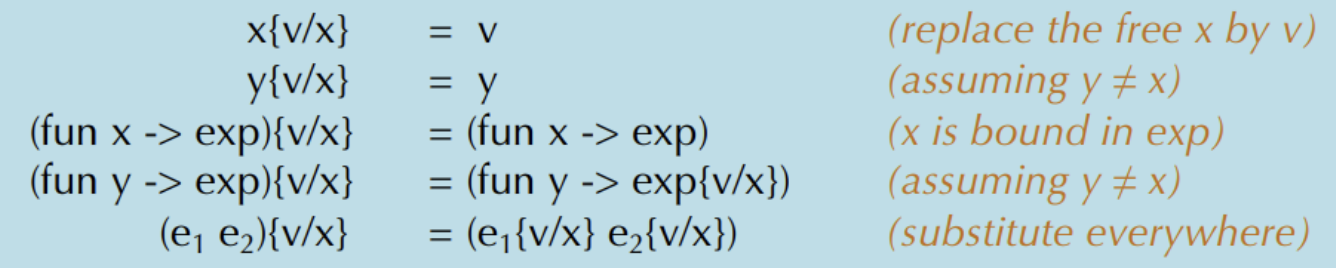
\includegraphics[width=\linewidth]{substitutions.png}
\end{center}
		
Function application is interpreted by substitution. In \texttt{fun y -> x + y}, \texttt{x} is said to be free and \texttt{y} is bound by \texttt{fun y}. \medskip

A term without free variables is \textbf{closed}, else it is \textbf{open}.
	
Two terms that differ only by consistent renaming of bound variables are alpha equivalent. \medskip

To avoid accidently capturing a free variable by a substitution $e_1 \{e_2 / x\}$, we first pick an alpha equivalent version of $e_1$ such that the bound variables do not mention the free variables of $e_2$.\medskip

Some special Lambda Calculus terms:
\begin{compactitem}
	\item Omega Term (infinite loop): 
	$$(\lambda x. x x)(\lambda x. x x)$$
	
	\item Y-Combinator (computes fixed point so $Yg = g(Yg)$): 
	$$\lambda f. (\lambda x. f(x, x))(\lambda x. f(x, x))$$
\end{compactitem}\medskip
	
Operational Semantics is a way to give meaning to a program (interpreter) using inference rules. $exp \Downarrow v$ means $exp$ evaluates to $v$. \medskip

Inference rules are of the form $G; L \vdash e : t$. This means in the global environment $G$ and local environment $L$ the expression $e$ is of type $t$. Sometimes we include a third symbol on the LHS referring to the return type. \medskip

With this we can build up derivation or proof trees. Leaves of the tree are axioms.
